\documentclass[main.tex]{subfiles}
\begin{document}

% \begin{extracontent}

\paragraph{Problem statement}
What happens if we impose the boundary condition that \(f(x_0, p)\) is not zero, but instead it equals the (small) background cosmic ray density in the galaxy?

The PDE system to solve for the phase space density \(f(x, p)\) is
%
\begin{align}
u_1 \pdv{f}{x} &= \pdv{}{x} \left( D \pdv{f}{x} \right)  \\
D \eval{\pdv{f}{x}}_{x=0^{-}} &= \frac{1}{3} (u_2 - u_1 ) p \eval{\pdv{f}{p}}_{x=0^{-}}  \\
f(x= x_0) &= g(p) = A \left( \frac{p}{p _{\text{min}}} \right)^{- \alpha  _{\text{CR}}}
\,.
\end{align}

\paragraph{Choice of ansatz}

Let us assume the solution looks like 
%
\begin{align}
f(x, p) \propto \exp(\frac{x u_1 }{D}) \left(\frac{p}{p _{\text{min}}}\right)^{- \beta (x)}
\,,
\end{align}
%
and for convenience let us rescale the position coordinate as \(X = x u_1 / D\).

There is an intrinsic problem in this approach: \(D\) is a function of \(p\), so treating it as constant does not capture the full behavior of the spectrum. 
The working idea here is that we are solving the equation only in small regions in \(p\) space, specifically ones where either \(X_0 = x_0 u_1 /D\) is much larger or much smaller than 1.
Then, we will join these solutions. 

Working through the derivatives, the terms related to the spatial exponential cancel, and the first equation upstream tells us that 
%
\begin{align}
(\beta ')^2 = \beta '' + \beta '
\,,
\end{align}
%
where primes denote derivatives with respect to \(X\),
while the condition at the shock tells us that 
%
\begin{align}
1 - \beta ' =  \frac{1}{3} \frac{r - 1 }{r}  \beta 
\,.
\end{align}

Finally, the condition at the \(X_0 = x_0 u_1 / D \) border tells us that 
%
\begin{align}
\beta (X = X_0 ) = \alpha _{\text{CR}}
\,
\end{align}
%
for some fixed \(\beta \). 

\paragraph{Numerical solution}

% The solution is basically as follows: when \(D / u_1 \ll \abs{x_0 }\) the spectral index \(\beta (x = 0)\) is basically \(3r/(r-1)\), while when \(D / u_1 \gg \abs{x_0 }\) the spectral index at \(x=0\) is basically the same as the one at \(x_0 \). 

% So, on a rough level in momentum space we expect a broken powerlaw spectrum, with index \(3r/(r-1)\) at low momenta and index \(\alpha _{\text{CR}}\) at high momenta, where the two are separated at \(p_*\) such that \(D(p_*) = u_1 \abs{x_0 }\). 

A numerical solution to this ODE is shown in figures \ref{fig:cosmic_ray_reacceleration_far} and \ref{fig:cosmic_ray_reacceleration_near}, for the cases of \(\abs{ X_0} \gg 1\) and \( \abs{X_0} \ll 1\) respectively. 

\begin{figure}[ht]
\centering
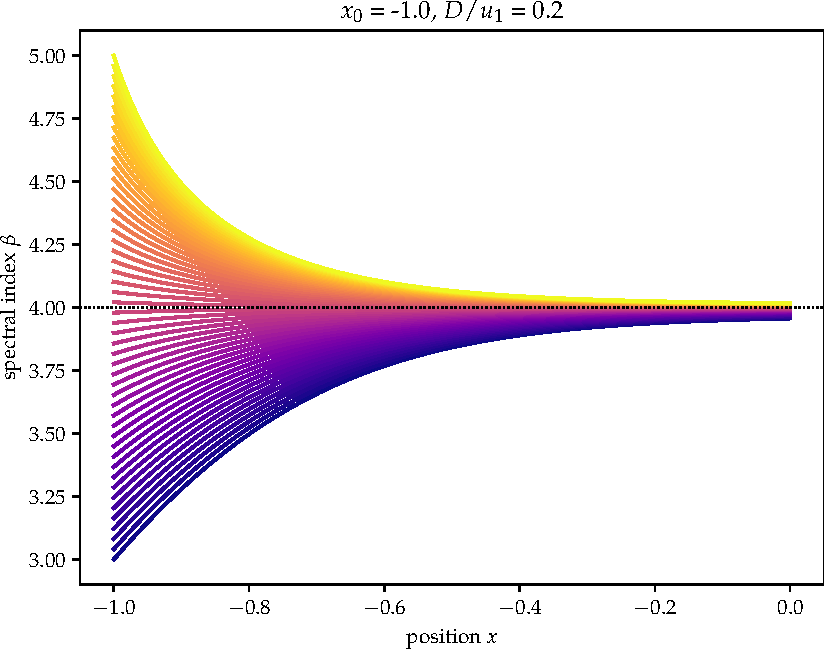
\includegraphics[width=\textwidth]{figures/cosmic_ray_reacceleration_far}
\caption{Reacceleration with \(D/u_1 \ll \abs{x_0 }\), or \(\abs{X_0} \gg 1 \) for various initial conditions.}
\label{fig:cosmic_ray_reacceleration_far}
\end{figure}

\begin{figure}[ht]
\centering
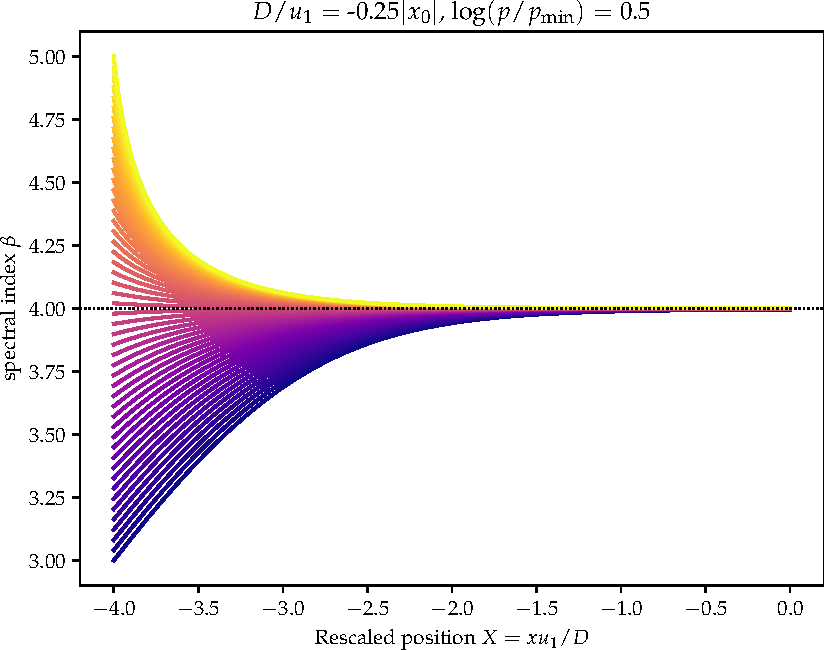
\includegraphics[width=\textwidth]{figures/cosmic_ray_reacceleration_near}
\caption{Reacceleration with \(D/u_1 \gg \abs{x_0 }\), or \(\abs{X_0 } \ll 1\) for various initial conditions.}
\label{fig:cosmic_ray_reacceleration_near}
\end{figure}

\paragraph{Analytical solution}

We can also solve the ODE for \(\beta \) explicitly; the ansatz
%
\begin{align}
\beta (X) = -\log (c_1 e^{X} + 1) + X + c_2 
\,,
\end{align}
%
solves it, as we can show explicitly: since \(\beta ' = -c_1 e^X /(c_1 e^X + 1) + 1\) 
and \(\beta '' = +c_1^2 e^{2X} / (c_1 e^X + 1)^2 - c_1 e^X / (c_1 e^X + 1) \), therefore 
%
\begin{align}
(\beta ')^2 - \beta '' &= \frac{c_1^2 e^{2X}}{(c_1 e^X + 1)^2} - 2 \frac{c_1 e^X}{c_1 e^X + 1} + 1  - \frac{c_1^2 e^{2X}}{(c_1 e^X + 1)^2} + \frac{c_1 e^X}{c_1 e^X + 1} \\
&= - \frac{c_1 e^X}{(c_1 e^X + 1)} + 1 = \beta '
\,.
\end{align}

The boundary conditions will fix \(c_1 \) and \(c_2 \): 
at \(x = x_0 \), meaning \(X= X_0 = x_0 u_1 / D \), we have \(\beta = \alpha _{\text{CR}}\), so 
%
\begin{align}
\alpha _{\text{CR}} = - \log (c_1 e^{X_0}  + 1) + X_0  + c_2
\,.
\end{align}

At \(X =0 \), on the other hand, we get 
%
\begin{align}
1 - \beta ' = \frac{c_1 e^X}{c_1 e^X + 1} &= \frac{1}{3} \frac{r-1}{r} \left( - \log \left( c_1 e^X + 1\right) + X + c_2  \right)  \\
\frac{c_1 }{c_1 + 1} &= \frac{1}{3} \frac{r-1}{r} \left( - \log (c_1 + 1) + c_2  \right)
\,.
\end{align}

The combination we actually want to compute is the one which gives the spectral index at \(X = 0\),
%
\begin{align}
\beta_0 = \beta (X = 0) = - \log (c_1 + 1) + c_2 
\,,
\end{align}
%
so we have 
%
\begin{align}
\beta_0 &= \frac{3r}{r-1} \frac{c_1 }{c_1 + 1}  \\
c_2 &= + \log (c_1 e^{X_0} + 1) - 1 + \alpha _{\text{CR}} \\
\beta_0 &= - \log (c_1 + 1 ) + c_2  \\
&= \log \frac{c_1 e^{X_0} + 1}{c_1 + 1} - X_0  + \alpha _{\text{CR}}
\,.
\end{align}

This also means we can make an equation for \(c_1 \) alone:
%
\begin{align}
c_2 &= \frac{3r}{r-1} \frac{c_1}{c_1 + 1} + \log(c_1 + 1)  \\
&= + \log (c_1 e^{X_0} + 1) - X_0  + \alpha _{\text{CR}}  \\
\alpha _{\text{CR}} &= + \frac{3r}{r-1} \frac{c_1}{c_1 + 1} + \log(c_1 + 1) - \log (c_1 e^{X_0} + 1) + X_0   \\
&= \underbrace{\frac{3r}{r-1} \frac{c_1}{c_1 + 1}}_{\beta_0 } + \log \frac{c_1 + 1}{c_1 + e^{-X_0 }}
\,.
\end{align}

% An admissible solution --- as long as the power spectral index given at the boundary is the same as the one at the shock (\(\alpha _{\text{CR}} = 3r/(r-1)\)) --- is \(\beta = \text{const}\).
% This corresponds to the \(c_1 \to \infty\) limit, with \(c_2 = \alpha _{\text{CR}}\).

If we are given \(X_0 \) and \(\alpha _{\text{CR}}\), we can (numerically) compute \(\beta_0\) by first computing the integration constant \(c_1 \) and then plugging it into the expression above. 

This equation makes intuitive sense in the \(X_0 \to 0\) limit: the logarithm approaches \(\log 1 = 0\), so we get \(\alpha _{\text{CR}} = \beta_0\). 
% \end{extracontent}

\paragraph{The broken powerlaw}

Zooming out, the behavior we expect is that for small momenta \(\abs{X_0} \ll 1 \) while for large momenta \(\abs{X_0 } \gg 1\), with the threshold being given by the \(p_*\) such that \(D(p_*) = u_1 \abs{x_0 }\). 

Then, what we expect to see is a broken powerlaw, with index \(\beta_0 = 3r / (r-1)\) in the low-momentum region and \(\beta_0 = \alpha _{\text{CR}}\) in the high-momentum region.

\end{document}